%%%%%%%%%%%%%%%%%%%%%%%%%%%%%%%%%%%%%%%%%
% Beamer Presentation
% LaTeX Template
% Version 1.0 (10/11/12)
%
% This template has been downloaded from:
% http://www.LaTeXTemplates.com
%
% License:
% CC BY-NC-SA 3.0 (http://creativecommons.org/licenses/by-nc-sa/3.0/)
%
%%%%%%%%%%%%%%%%%%%%%%%%%%%%%%%%%%%%%%%%%

%----------------------------------------------------------------------------------------
%	PACKAGES AND THEMES
%----------------------------------------------------------------------------------------

\documentclass{beamer}

\mode<presentation> {

% The Beamer class comes with a number of default slide themes
% which change the colors and layouts of slides. Below this is a list
% of all the themes, uncomment each in turn to see what they look like.

%\usetheme{default}
%\usetheme{AnnArbor}
%\usetheme{Antibes}
%\usetheme{Bergen}
%\usetheme{Berkeley}
%\usetheme{Berlin}
%\usetheme{Boadilla}
%\usetheme{CambridgeUS}
%\usetheme{Copenhagen}
%\usetheme{Darmstadt}
%\usetheme{Dresden}
%\usetheme{Frankfurt}
%\usetheme{Goettingen}
%\usetheme{Hannover}
%\usetheme{Ilmenau}
%\usetheme{JuanLesPins}
%\usetheme{Luebeck}
\usetheme{Madrid}
%\usetheme{Malmoe}
%\usetheme{Marburg}
%\usetheme{Montpellier}
%\usetheme{PaloAlto}
%\usetheme{Pittsburgh}
%\usetheme{Rochester}
%\usetheme{Singapore}
%\usetheme{Szeged}
%\usetheme{Warsaw}

% As well as themes, the Beamer class has a number of color themes
% for any slide theme. Uncomment each of these in turn to see how it
% changes the colors of your current slide theme.

%\usecolortheme{albatross}
%\usecolortheme{beaver}
%\usecolortheme{beetle}
%\usecolortheme{crane}
\usecolortheme{dolphin}
%\usecolortheme{dove}
%\usecolortheme{fly}
%\usecolortheme{lily}
%\usecolortheme{orchid}
%\usecolortheme{rose}
%\usecolortheme{seagull}
%\usecolortheme{seahorse}
%\usecolortheme{whale}
%\usecolortheme{wolverine}

%\setbeamertemplate{footline} % To remove the footer line in all slides uncomment this line
\setbeamertemplate{footline}[page number] % To replace the footer line in all slides with a simple slide count uncomment this line

%\setbeamertemplate{navigation symbols}{} % To remove the navigation symbols from the bottom of all slides uncomment this line
}

\usepackage{graphicx} % Allows including images
\usepackage{booktabs} % Allows the use of \toprule, \midrule and \bottomrule in tables
\usepackage[absolute,overlay]{textpos}
\usepackage{multicol}
\usepackage{pseudocode}

%\hypersetup{
%	colorlinks = true,
%	linkcolor = red
%}

%\makeatletter
%\let\@mycite\@cite
%\def\@cite#1#2{{\hypersetup{linkcolor=green!60!black}[{#1\if@tempswa , #2\fi}]}}
%\makeatother



%----------------------------------------------------------------------------------------
%	TITLE PAGE
%----------------------------------------------------------------------------------------

\title[Interring programs structure from an execution trace]
{
	\textit{Master thesis} \\
	Master in Research and Innovation \\
	\vspace{0.5cm}
	%\hrulefill \\
	\textbf{Inferring programs structure from \\
		an execution trace} \\
	%\hrulefill \\
}

\author
{%
	\texorpdfstring{
	\begin{multicols}{2}
		{\small \textit{Author}}\\
		Juan Francisco Mart\'inez Vera\\
		\columnbreak
		{\small \textit{Supervisor}}\\
		Jes\'us Labarta Mancho\\
	\end{multicols}
	}
	{ }
}
\institute[FIB, UPC]
{
	Facultat d'Inform\`atica de Barcelona (FIB) \\
	Universitat Polit\`ecnica de Catalunya (UPC)
	\begin{figure}
		
\includegraphics[width=30px]{imgs/logo_upc.png}
	\end{figure}
}
\date{\today}

\AtBeginSection[]
{
	\begin{frame}<beamer>
		\frametitle{Outline for section \thesection}
		\tableofcontents[currentsection]
	\end{frame}
}

\begin{document}
%\logo{
\includegraphics[height=0.5cm]{imgs/logo_upc.png}}

\begin{frame}
\titlepage
\end{frame}

\begin{frame}[allowframebreaks]
\frametitle{Presentation outline}
\tableofcontents
\end{frame}

%----------------------------------------------------------------------------------------
%	PRESENTATION SLIDES
%----------------------------------------------------------------------------------------

\section{Context}
%\subsection{High Performance Computing}
%\begin{frame}
%\frametitle{High Performance Computing}
%\begin{itemize}
%	\item Becomes the third support of science with mathematics and theory
%	\item Tremendous improvement in all transformation hierarchy layers
%\end{itemize}
%\begin{figure}
%	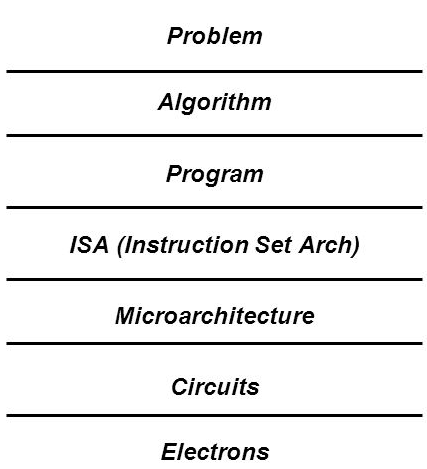
\includegraphics[width=100px]{imgs/transformationhierarchy.png}
%	\caption{Transformation hierarchy}
%\end{figure}
%\begin{textblock*}{5cm}(40px,160px) % {block width} (coords)
%	\includegraphics<+(1)->[width=70px]{imgs/moore_prediction.png}
%\end{textblock*}
%\begin{textblock*}{5cm}(40px,100px) % {block width} (coords)
%	\includegraphics<+(1)->[width=70px]{imgs/microarchitecture.png}
%\end{textblock*}
%\begin{textblock*}{5cm}(270px,170px) % {block width} (coords)
%	\includegraphics<+(1)->[width=70px]{imgs/multicore.png}
%\end{textblock*}
%\begin{textblock*}{5cm}(270px,100px) % {block width} (coords)
%	\includegraphics<+(1)->[width=70px]{imgs/program_simulation.png}
%\end{textblock*}
%\end{frame}

\subsection{Performance Analysis tools}
\begin{frame}
\frametitle{Performance Analysis tools (i)}
\begin{itemize}
%	\item Focused on Program layer
	\item Aid to detect bottlenecks
	\item Is a cyclic process
	\begin{itemize}
%		\item Less iterations better
		\item \# iterations depens on quality of hypothesis
		\item That is strongly related with possibilities tools provides
	\end{itemize}
	\item Analyst have to work with codes \textbf{they are not familiar with}
	\begin{itemize}
		\item POP project
		\item \textbf{Syntactic structure help analyst} to understand what is going on
	\end{itemize}
\end{itemize}
\begin{multicols}{2}
	\begin{figure}
		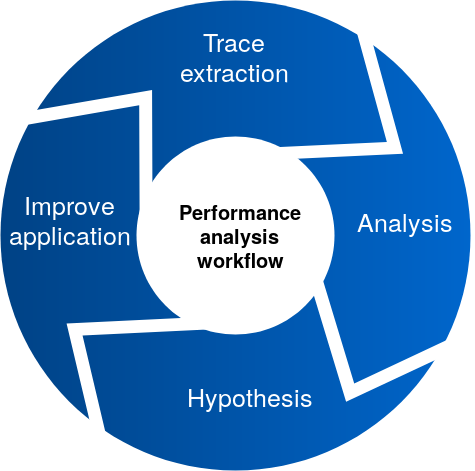
\includegraphics[height=80px]{imgs/performance_analysis_diagram.png}
		\caption{Performance analysis workflow}
	\end{figure}
	\columnbreak

	\begin{figure}
		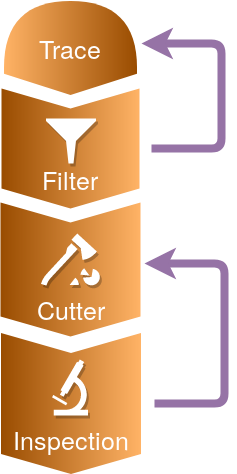
\includegraphics[height=80px]{imgs/analysis_subphases.png}
		\caption{Analysis subphases}
	\end{figure}
\end{multicols}
\end{frame}

\section{State of the Art}

\begin{frame}
\frametitle{State of the Art}
	Previous research on syntactic structure\\
	\begin{itemize}
		\item Previous research have been driven in this field.
		\item Since traces are ordered sequences...
		\item ... Natural choice has been \textbf{sequential pattern mining} in general.
	\end{itemize}
	As main drawback\\
	\begin{itemize}
		\item This sort of algorithms, \textbf{used to present high complexity}.
		\item From $O(n^{2})$ to $O(2^{n})$.
	\end{itemize}
\end{frame}

\section{Motivations}
\begin{frame}
\frametitle{Motivations}
\begin{block}{Motivation 1: About improve understandability...}
	Providing application structure will lead to better understandability about what the application is doing.
\end{block}
\pause
\begin{block}{Motivation 2: About identify regions of interest...}
	Having the structure of the application can aid the process of identify regions of interest
\end{block}
\pause
\begin{block}{Motivation 3: About been scalable...}
	Because the trend of increasing trace sizes, explore an alternative to improve scalability. 
\end{block}
\end{frame}

\section{Proposal}
\subsection{Application structure by classification}
\begin{frame}
\frametitle{Application structure by classification}
\framesubtitle{Intuition}
HPC applications idiosincracy\\
\begin{itemize}
	\item Big outer loop
	\item Repetitive and stable executions
	\item Communications lies on loops that drives the execution
\end{itemize}
Taking this into account...\\
\begin{itemize}
	\item Stable executions implies \textbf{similar behaviour for all iterations} in a given loop
	\item Loops can be discovered by \textbf{monitoring the communications}.
	\item So...
\end{itemize}
\vfill
\pause
\begin{block}{The key idea}
	Communications are used as \textbf{proxies} for the observation of iterations. Clustering them \textbf{by its behaviour} the applications structures can be betrayed.
\end{block}
\end{frame}

\begin{frame}
\frametitle{Application structure by classification}
\framesubtitle{Defining behaviour}
Selected features must be able to
\begin{itemize}
	\item Join MPIs from the same loop
	\item Separe MPIs from different loops
\end{itemize}
\vfill
\pause
As a starting point ...
\begin{enumerate}
	\item \textbf{Number of repetitions}: Two different mpi calls in same loop will be executed the same ammount of time
	\item \textbf{Mean time between repetitions}: Two different loops will, presumibly, execute different work
\end{enumerate}
\end{frame}

\subsection{Workflow}
\begin{frame}
\frametitle{Workflow}
\begin{figure}
	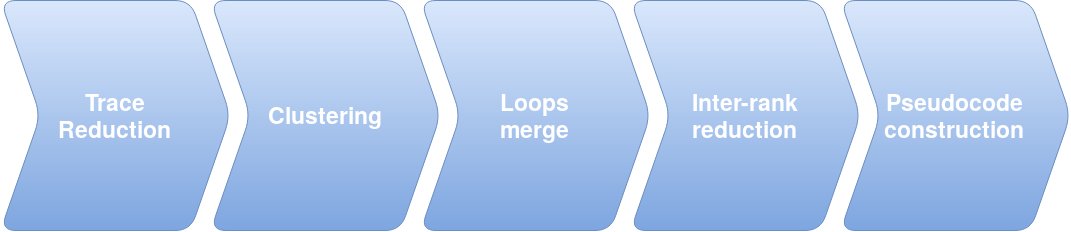
\includegraphics[width=\textwidth]{imgs/workflow.png}
	\caption{Structure detection workflow}
\end{figure}
\end{frame}

\begin{frame}
\frametitle{Workflow}
\framesubtitle{Trace reduction step (i)}
\textbf{Input} Tracefile, i.e. Sequence of timestamped events ordered by time.\\
\textbf{Output} Set of unique MPI calls with attached information.
\vspace{10px}
\pause
\begin{itemize}
	%\item By \textbf{reduction} and \textbf{aggregation \& derivation}
	\item Is a sort of Map \& Reduce
	\item Every MPI call is identified by its \textbf{signature}
	\item Being the signature: Ordered sequence of pairs $(file,line)$ that define the call path, i.e. The dynamic position
\end{itemize}
\pause
\begin{figure}
	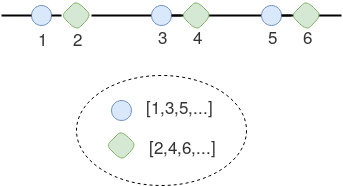
\includegraphics[width=0.5\textwidth]{imgs/workflow_reduction.png}
\end{figure}
\end{frame}

\begin{frame}
\frametitle{Workflow}
\framesubtitle{Trace reduction step (ii)}
Additionally \textbf{filter less representative MPI calls}.
\begin{itemize}
	\item Allows to decrease even more the clustering complexity.
	\item Focus only on the important data (normally set to 10\%).
	\item The criteria is whether a given threshold of ``explained time'' is surpased.
\end{itemize}
\begin{equation}
	\delta(call) = \frac{it(call)*imt(call)}{T_{exe}}
\end{equation}
\begin{figure}
	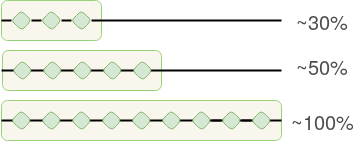
\includegraphics[width=0.5\textwidth]{imgs/workflow_reduction_2.png}
\end{figure}
\end{frame}

\begin{frame}
\frametitle{Workflow}
\framesubtitle{Trace reduction step (iii)}
The stored information for every unique MPI call is:
\begin{itemize}
	\item \textbf{Number of repetitions}
	\item Timestamps $\rightarrow$ \textbf{Mean time time between repetitions}
	\item Entire call path
	\item Previous burst performance information
	\item Calculed delta
\end{itemize}
\vfill
\pause
\begin{block}{The key point for scalability}
	HPC applications are strongly repetitive over time so number of unique MPI calls will remain despite the increasing problem size.
\end{block}
\end{frame}

\begin{frame}
\frametitle{Workflow}
\framesubtitle{Clustering}

\textbf{Input} Set of unique MPI calls with attached information.\\
\textbf{Output} Set of sets of MPI calls.
\vspace{10px}
\pause

\begin{itemize}
	\item \textbf{DBSCAN} as clustering algorithm (prefered to K-means)
	\begin{itemize}
		\item $\epsilon$ empirically set to 0.2 (in general)
		\item minPts set to 1
		\item Number of repetitions vs. Mean time between repetitions
	\end{itemize}
\pause
	\item Resulting clusters \textbf{will be considered loops}.
	\begin{itemize}
		\item Since MPI calls acts as proxies
		\item Number of repetitions $\rightarrow$ Number of iterations.
		\item Mean time between repetitions $\rightarrow$ Mean iterations time.
	\end{itemize}
\end{itemize}
\pause
\begin{multicols}{2}
	\begin{figure}
		\includegraphics[width=0.3\textwidth,height=0.3\textheight]{imgs/clustering_ex_1.png}
	\end{figure}
	\begin{figure}
		\includegraphics[width=0.3\textwidth,height=0.3\textheight]{imgs/clustering_ex_2.png}
	\end{figure}
\end{multicols}
\end{frame}

\begin{frame}
\frametitle{Workflow}
\framesubtitle{Loops merge (i)}
\textbf{Input} Set of loops.\\
\textbf{Output} Set of top level loops with its related nested loops.\\
\vspace{10px}
\pause
Intuition
\begin{itemize}
	\item Isolated loops are just \textbf{pieces of the overall puzzle}.
	\item By discover its hierarchical relations \textbf{the structure of the application will be betrayed}.
\end{itemize}
\pause
Some clues
\begin{itemize}
	\item Outer loop will have \textbf{less iterations} than nested one.
	\item Outer loop will spend \textbf{more time} per iteration.
	%\item Outer loop will \textbf{explain the same amount of time} as inner loop.
\end{itemize}
\end{frame}

\begin{frame}
\frametitle{Workflow}
\framesubtitle{Loops merge (ii)}
\begin{multicols}{2}
%	\begin{pseudocode}{ }{ }
%		\FOR 1 \text{ to } 10 \DO
%		\BEGIN
%			\FOR 1 \text{ to } 2 \DO
%			\BEGIN
%				\FOR 1 \text{ to } 2 \DO
%				\BEGIN
%					MPI\_Call() \\
%				\END\\
%				MPI\_Call()\\
%			\END \\
%			MPI\_Call()\\
%		\END\\
%		\FOR 1 \text{ to } 100 \DO
%		\BEGIN
%			\FOR 1 \text{ to } 2 \DO
%			\BEGIN
%				\FOR 1 \text{ to } 2 \DO
%				\BEGIN
%					MPI\_Call() \\
%				\END\\
%				MPI\_Call()\\
%			\END \\
%			MPI\_Call()\\
%		\END
%	\end{pseudocode}
	\begin{figure}
		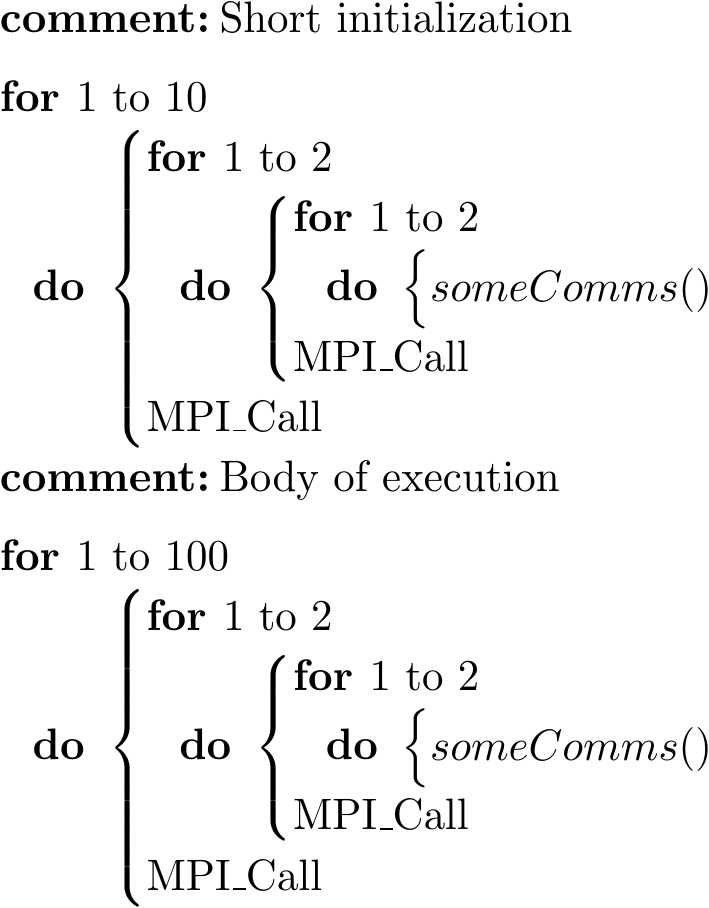
\includegraphics[width=0.25\textwidth]{imgs/delta_clustering_test_1_pse.png}
	\end{figure}
	\columnbreak
	\begin{figure}
		\includegraphics[width=0.4\textwidth]<1>{imgs/clustering_ex_2_2.png}
		\includegraphics[width=0.4\textwidth]<2->{imgs/delta_clustering_test_1.png}
	\end{figure}
\end{multicols}
\begin{itemize}
	\item $O(\frac{n^{2}-n}{2}) \approx O(n^{2})$ comparissons
	\pause
	\item Reduce search space by classify loops by its delta
	\begin{itemize}
		\item All lies on same $f(x)=\frac{\delta*T_{exe}}{x}$ being $0 < \delta < 1$
	\end{itemize}
	\item And then merge them in a less to more iterations fashion
\end{itemize}
\pause
\begin{block}{Keynote}
	This mechanism is then used for phases detection as well.
\end{block}
\end{frame}

%\begin{frame}
%\frametitle{Workflow}
%\framesubtitle{Loops merge (iii)}
%\begin{multicols}{2}
%	\begin{figure}
%		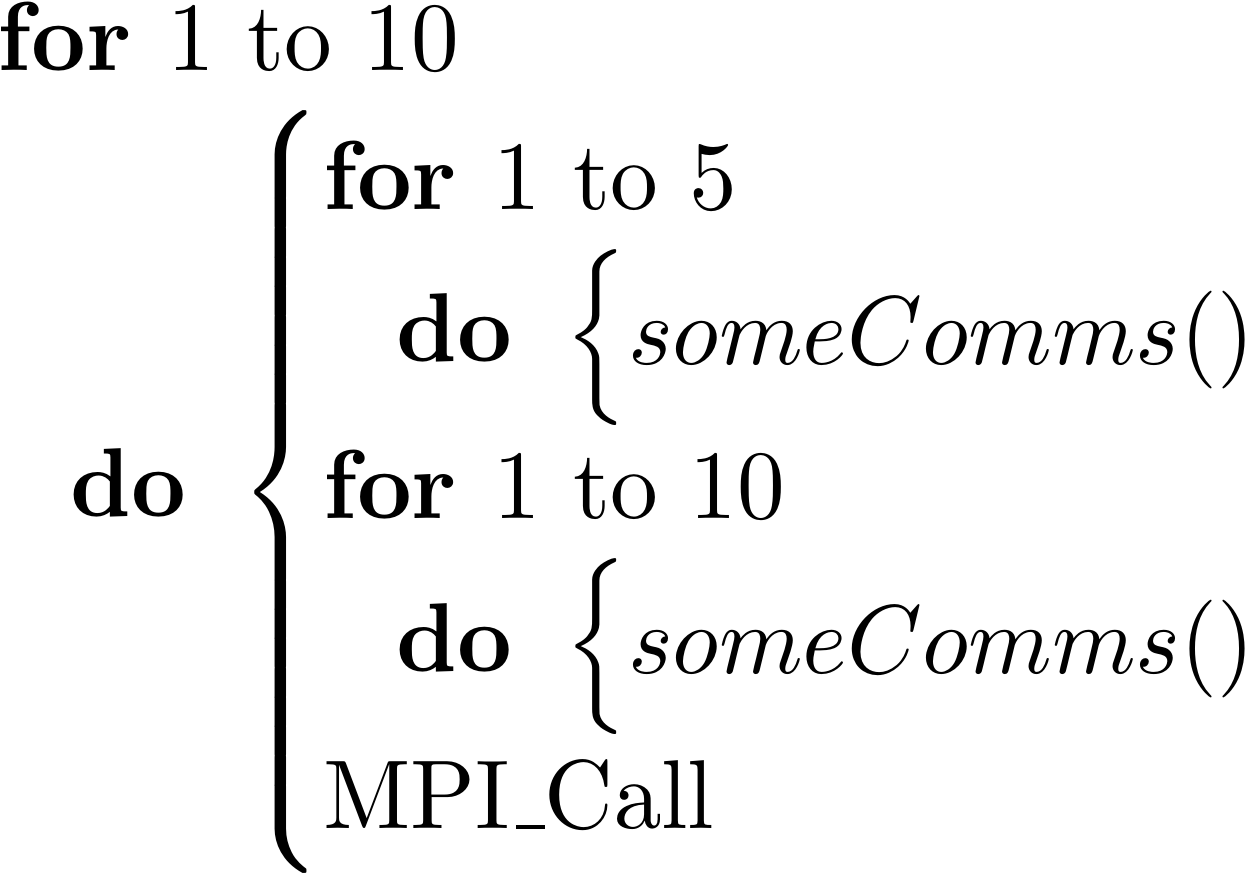
\includegraphics[width=0.4\textwidth]{imgs/delta_clustering_test_2_pse.png}
%	\end{figure}
%	\pause
%	\columnbreak
%	\begin{figure}
%		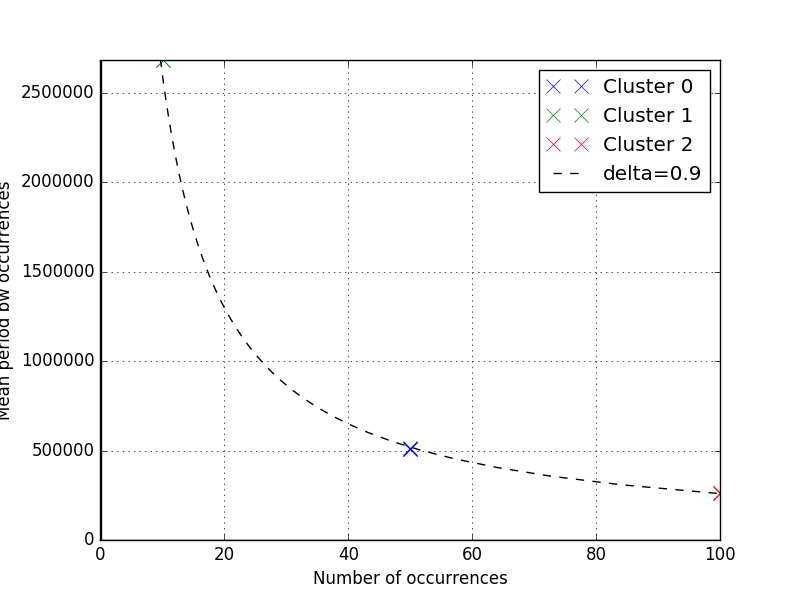
\includegraphics[width=0.5\textwidth]{imgs/delta_clustering_test_2.png}
%	\end{figure}
%\end{multicols}
%\pause
%\begin{block}{Warning}
%	Not all loops that fulfills with nested loops conditions, are nested loops.\\
%	Extra check is needed.
%\end{block}
%\end{frame}

%\begin{frame}
%\frametitle{Workflow}
%\framesubtitle{Loops merge (iv)}
%\begin{itemize}
%	\item Classify MPI clusters/Loops ($\upsilon \in \Upsilon$) per ``how much of execution represents'' ($\delta \in \Delta$)\footnote{Do not confuse with $\delta()$ function.}.
%	\item For every phase ($\delta$) sort loops ($\upsilon$) by number of iterations.
%	\item Perform the loop merge \textbf{from high to low iterations count}.
%	\item Before every merge, \textbf{check out} whether the hierarchical relationship is true.
%\end{itemize}
%\begin{figure}
%	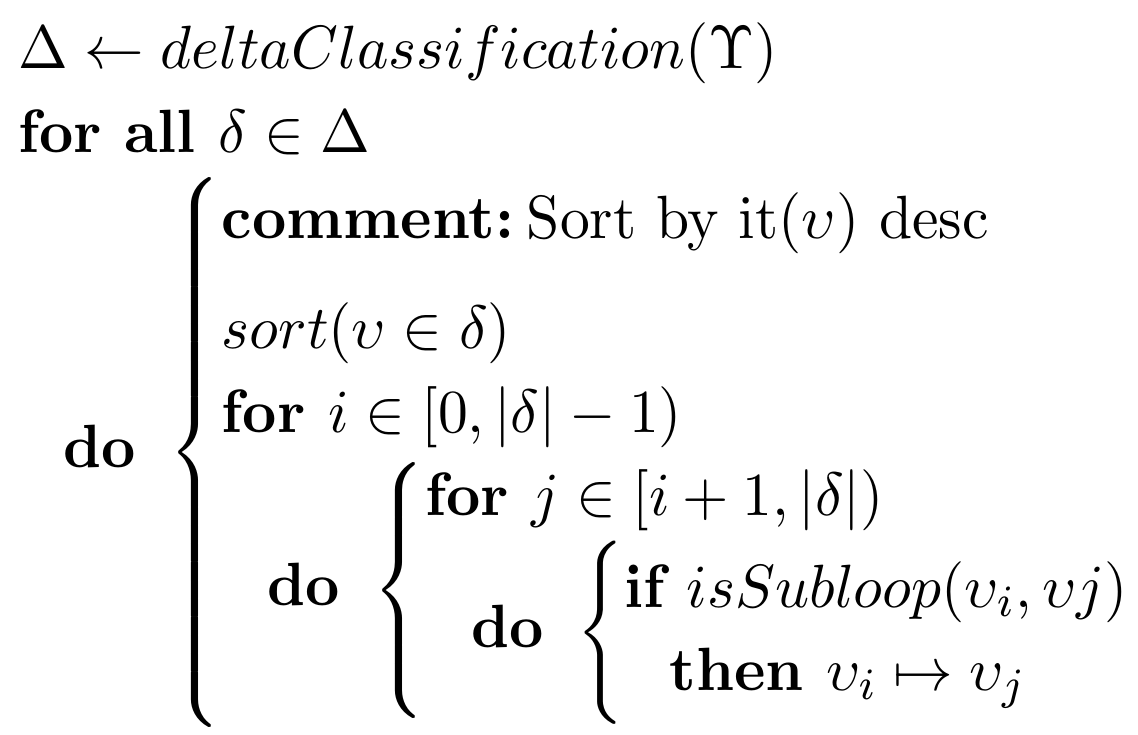
\includegraphics[width=0.5\textwidth]{imgs/loops_merge_pseudocode.png}
%\end{figure}
%\end{frame}

\begin{frame}
\frametitle{Workflow}
\framesubtitle{Inter-rank reduction (i)}
\textbf{Input} Set of top level loops.\\
\textbf{Output} Set of top level loops with rank conditional structures.\\
\vspace{10px}
\pause
\begin{itemize}
	\item Two calls with \textbf{same call paths still coexist} if belongs to different MPI ranks.
	\begin{itemize}
		\item \textbf{Conservative} reduction step!
	\end{itemize}
	\item Divergences between MPI ranks are understood as \textbf{conditional structures in code}.
	\item This step is about: 
	\begin{enumerate}
		\item MPI Calls/Subloops ordenation
		\item Reduction
		\item Arrangement in conditional blocks
	\end{enumerate}
\end{itemize}
\pause
\begin{block}{Idea}
	Inter-rank reduction step could be moved to the actual Reduction step, leaving this workflow step just for conditional blocks construction.
\end{block}
\end{frame}

%\begin{frame}
%\frametitle{Workflow}
%\framesubtitle{Inter-rank reduction (ii)}
%
%	\begin{enumerate}
%		\item [0] main() : 10 $>$ B() : 2 $>$ MPI
%		\item [1] main() : 10 $>$ B() : 2 $>$ MPI
%		\item [0] main() : 10 $>$ B() : 5 $>$ C() : 7 $>$ MPI
%		\item [1] main() : 10 $>$ B() : 5 $>$ C() : 8 $>$ MPI
%		\item [0] main() : 10 $>$ C() : 2 $>$ MPI
%		\item [1] main() : 10 $>$ C() : 2 $>$ MPI
%	\end{enumerate}
%	\pause
%	\begin{enumerate}
%		\item [0,1] main() : 10 $>$ B() : 2 $>$ MPI
%		\item [0] main() : 10 $>$ B() : 5 $>$ C() : 7 $>$ MPI
%		\item [1] main() : 10 $>$ B() : 5 $>$ C() : 8 $>$ MPI
%		\item [0,1] main() : 10 $>$ C() : 2 $>$ MPI
%	\end{enumerate}
%\end{frame}

\begin{frame}
\frametitle{Workflow}
\framesubtitle{Pseudocode construction (i)}
\textbf{Input} Set of top level loops with rank conditional structures.\\
\textbf{Output} Pseudocode representing the actual application structure. \\
\vspace{5px}
\pause
\begin{itemize}
	\item Straightforward construction
	\item For bettern understanding \textbf{repetitive information from call paths is removed}.
	\begin{enumerate}
		\item Extracting common call path levels from code block (loops and conditional blocks)
		\item Removing \textbf{contiguous repetitive information} what has not been removed in previous step
	\end{enumerate}
\end{itemize}
\begin{multicols}{3}
	\begin{figure}
		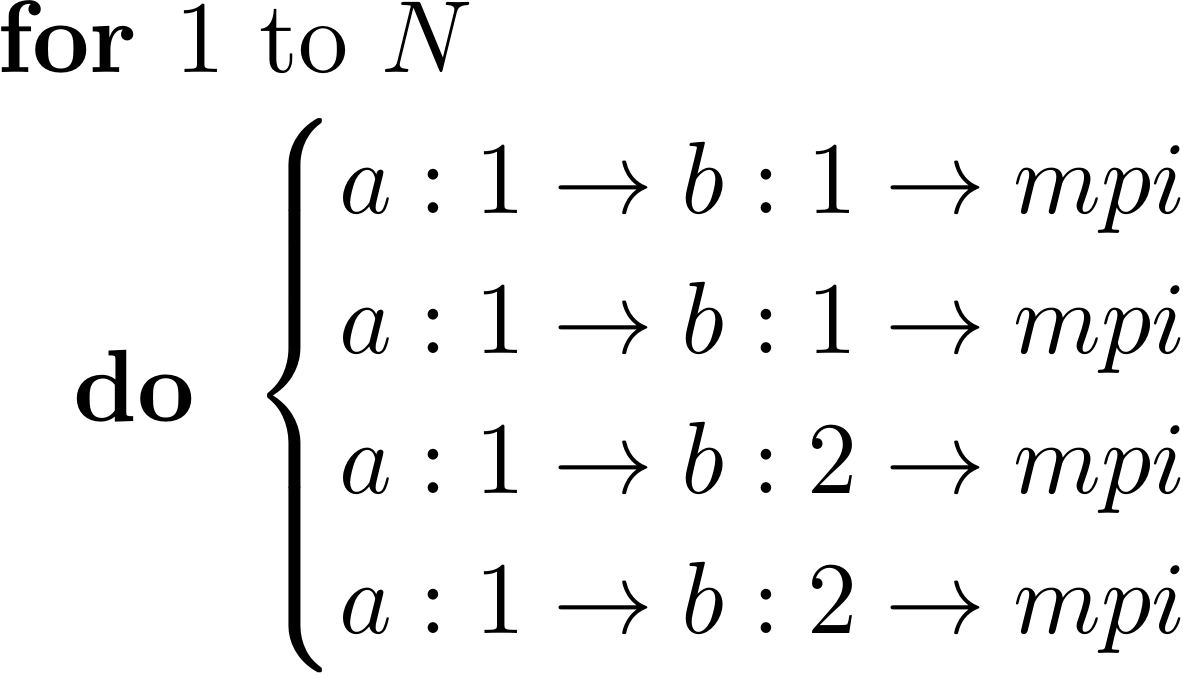
\includegraphics[width=0.3\textwidth]{imgs/workflow_pseudocode_1.png}
		\caption{Raw pseudocode}
	\end{figure}
	\columnbreak
	\pause
	\begin{figure}
		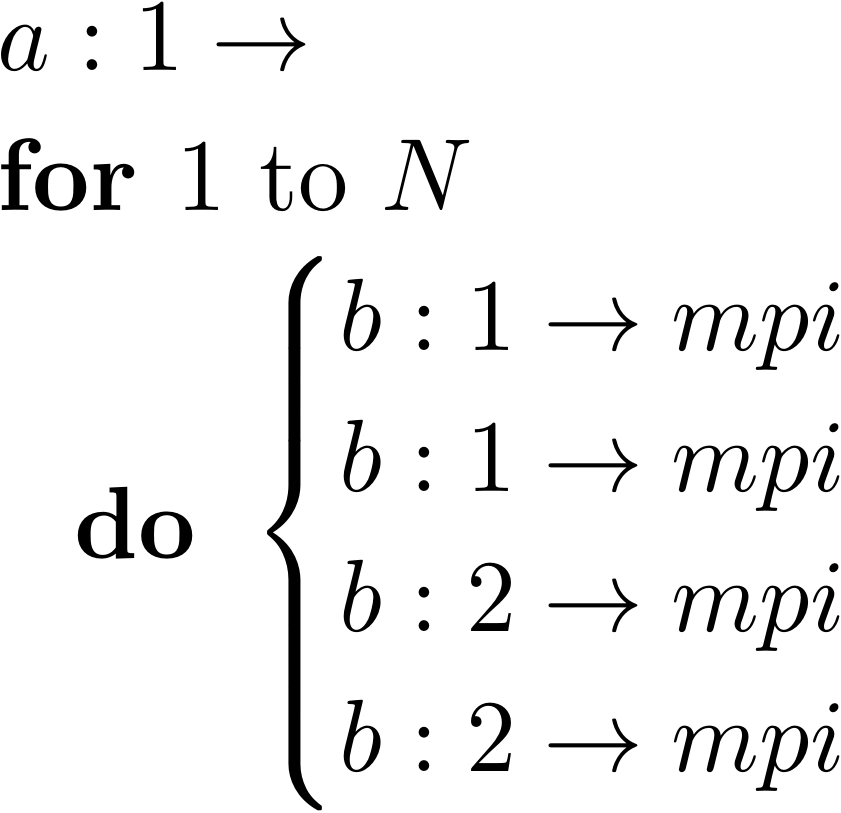
\includegraphics[width=0.18\textwidth]{imgs/workflow_pseudocode_2.png}
		\caption{After extract common call path}	
	\end{figure}
	\columnbreak
	\pause
	\begin{figure}
		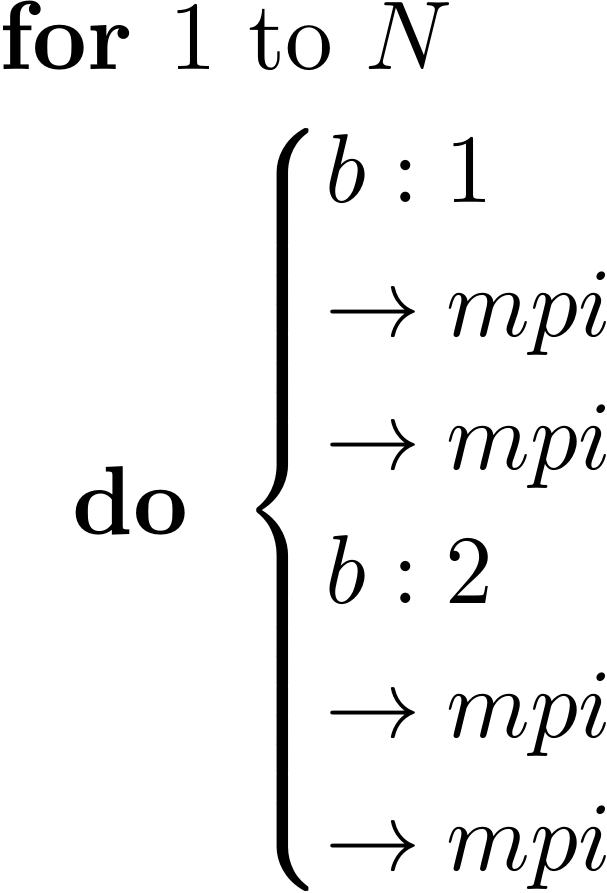
\includegraphics[width=0.14\textwidth]{imgs/workflow_pseudocode_3.png}
		\caption{After extract contiguous call path}
	\end{figure}
	\columnbreak
\end{multicols}
\end{frame}

\begin{frame}
\frametitle{Workflow}
\framesubtitle{Pseudocode construction (ii)}
\begin{figure}
	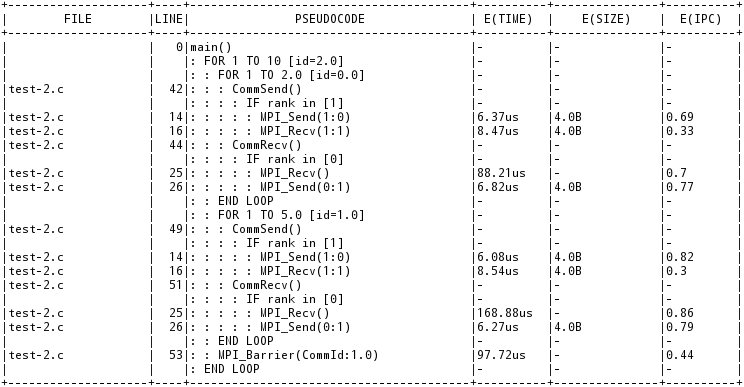
\includegraphics[width=0.7\textwidth]{imgs/console_gui_example_1.png}
	\caption{Example console output}
\end{figure}
\pause
\begin{itemize}
	\item Additionally an \textbf{interactive shell} is provided to the user allowing...
	\begin{enumerate}
		\item Show cpu burst metrics over a given thresshold.
		\item Filter by MPI rank.
		\item Show clustering plot.
		\item ...
	\end{enumerate}
\end{itemize}
\end{frame}

\section{Further considerations}
\begin{frame}
\frametitle{Further considerations}

Until now were not aware about \textbf{the problems can arise from clustering step}. \\
But there are some:
\begin{enumerate}
	\item \textbf{Cluster aliasing} when two different loops behaves similarly enough over our defined space
	\item \textbf{Hidden superloop} when not detected superloop prevents from a good structure detection.
	\item \textbf{Cluster split} when MPI calls belonging to the same loop behaves in a different way.
\end{enumerate}
\vfill
%\pause
%\begin{multicols}{2}
%	\begin{figure}
%		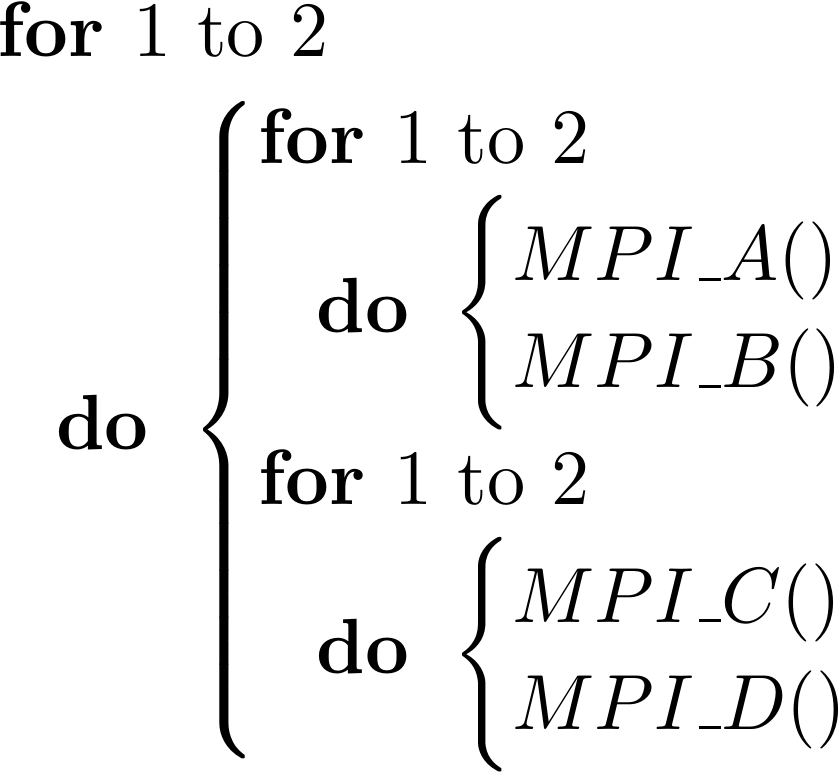
\includegraphics[height=80px]{imgs/aliasing_example.png}
%		\caption{Cluster aliasing example}
%	\end{figure}
%	\columnbreak
%	\begin{figure}
%		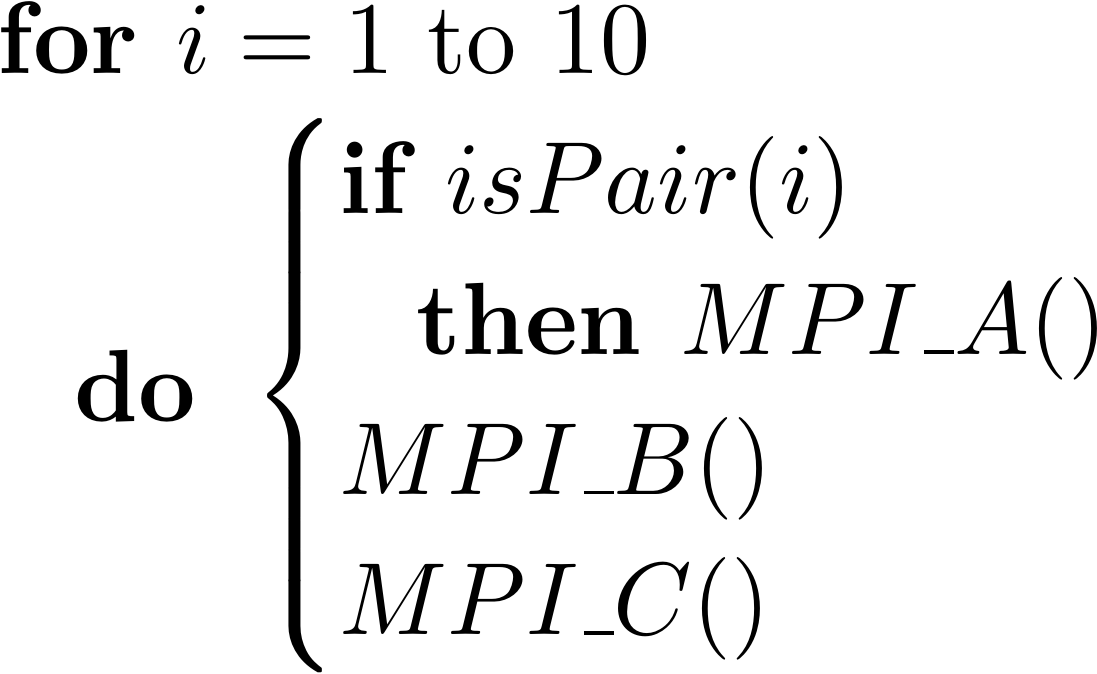
\includegraphics[height=80px]{imgs/split_example.png}
%		\caption{Cluster split example}
%	\end{figure}
%\end{multicols}
\end{frame}

\subsection{Proposal modifications}
\begin{frame}
\frametitle{Proposal modifications}
\framesubtitle{Cluster aliasing}
In the same loop, MPI calls are somehow interleaved
\begin{itemize}
	\item Imagine one loops containing $A$ and $B$ calls
	\item No aliasing: $A \rightarrow B \rightarrow A \rightarrow B \rightarrow A \rightarrow B$
	\item Aliasing: $A \rightarrow A \rightarrow A \rightarrow B \rightarrow B \rightarrow B$ 
\end{itemize}
\begin{multicols}{3}
	\begin{pseudocode}{ }{ }
		\FOR 1 to 2 \DO
		\BEGIN
			MPI\_A()\\
			MPI\_B()\\
		\END\\
		\FOR 1 to 2 \DO
		\BEGIN
			MPI\_A()\\
			MPI\_B()\\
		\END
	\end{pseudocode}
	\vfill \null
	\columnbreak
	\pause
	\null \vfill
	\begin{table}[]
		\centering
		\begin{tabular}{l|ll}
			MPI\_A & 1 & 3 \\
			MPI\_B & 2 & 4 \\
			MPI\_C & 5 & 7 \\
			MPI\_D & 6 & 8
		\end{tabular}
	\end{table}
	%\includegraphics[height=0.2\textheight]{imgs/cluster_aliasing_1.png}
	\vfill \null
	\columnbreak
	\pause
	\null \vfill
	\begin{table}[]
		\centering
		\begin{tabular}{l|llll}
			MPI\_A & 1 & 3 &   &   \\
			MPI\_B & 2 & 4 &   &   \\ \hline
			MPI\_C &   &   & 5 & 7 \\
			MPI\_D &   &   & 6 & 8
		\end{tabular}
	\end{table}
	%\includegraphics[height=0.2\textheight]{imgs/clustering_aliasing_2.png}
	\vfill \null
\end{multicols}
\end{frame}

\begin{frame}
\frametitle{Proposal modifications}
\framesubtitle{Hidden superloop}
The model will not detect loops w/o MPI calls
Can leads to bad results if more than one nested loops
\begin{itemize}
	\item Aliasing will be detected, but two 4-iteration loops
	\item Wrong: $A \rightarrow A \rightarrow A \rightarrow A \rightarrow B \rightarrow B \rightarrow B \rightarrow B$
	\item Correct: $A \rightarrow A \rightarrow B \rightarrow B \rightarrow A \rightarrow A \rightarrow B \rightarrow B$
\end{itemize}
\begin{multicols}{2}
	\begin{pseudocode}{ }{ }
		\FOR 1 to 2 \DO
		\BEGIN
			\FOR 1 to 2 \DO
			\BEGIN
				MPI\_A()\\
			\END\\
			\FOR 1 to 2 \DO
			\BEGIN
				MPI\_B()\\
			\END
		\END
	\end{pseudocode}
	\pause
	\columnbreak
	\begin{table}[]
		\centering
		\begin{tabular}{l | llll}
			MPI\_A & 1 & 2 & 5 & 6 \\ 
			MPI\_B & 3 & 4 & 7 & 8
		\end{tabular}
	\end{table}
	\pause
	\begin{table}[]
	\centering
	\begin{tabular}{l | llllllll}
		MPI\_A & 1 & 2 &   &   & 5 & 6 &   &   \\ \hline
		MPI\_B &   &   & 3 & 4 &   &   & 7 & 8
	\end{tabular}
	\end{table}
\end{multicols}
\end{frame}

%\begin{frame}
%\frametitle{Proposal modifications}
%\framesubtitle{Cluster split (i)}
%Whether MPI call is conditioned
%\begin{itemize}
%	\item \#repetitions and mean time bw. reps. change (in same proportion).
%\end{itemize} 
%\begin{multicols}{2}
%	\begin{pseudocode}{ }{ }
%		\FOR i=1 \text{ to } 10 \DO
%		\BEGIN
%			\IF isPair(i) \THEN
%				MPI\_A()\\
%			MPI\_B()\\
%		\END
%	\end{pseudocode}
%	\columnbreak
%	\begin{figure}
%		\includegraphics[width=0.3\textwidth]<1>{imgs/clustering_val_8_1.png}
%		\includegraphics[width=0.3\textwidth]<2>{imgs/clustering_val_8.png}
%	\end{figure}
%\end{multicols}
%\pause
%	\begin{figure}
%		\includegraphics[height=0.3\textheight]{imgs/result_val_8.png}
%	\end{figure}
%\end{frame}

\begin{frame}
\frametitle{Proposal modifications}
\framesubtitle{Cluster split}
Whether MPI call is conditioned
\begin{itemize}
	\item \#repetitions and mean time bw. reps. change (in same proportion).
\end{itemize} 
\begin{multicols}{2}
	\begin{figure}
		\includegraphics[height=60px]{imgs/split_example_2.png}
	\end{figure}
%	\begin{pseudocode}{ }{ }
%		\FOR i=1 \text{ to } 10 \DO
%		\BEGIN
%		MPI\_B()\\
%		\IF isPair(i) \THEN
%			MPI\_A()\\
%		MPI\_B()\\
%		\END
%	\end{pseudocode}
	\columnbreak
	\begin{figure}
		\includegraphics[width=0.3\textwidth]<1>{imgs/clustering_val_8_1.png}
		\includegraphics[width=0.3\textwidth]<2>{imgs/clustering_val_8.png}
	\end{figure}
\end{multicols}
\pause
By ``reverse loop merging'' and times checking
\begin{figure}
	\includegraphics[height=0.3\textheight]{imgs/result_val_9.png}
\end{figure}
\end{frame}
%	\begin{pseudocode}{ }{ }
%	\FOR i=1 \text{ to } 10 \DO
%	\BEGIN	
%	MPI\_B()\\
%	\IF isPair(i) \THEN
%	MPI\_A()\\
%	MPI\_B()\\
%	\END
%\end{pseudocode}

\subsection{Data analysis}
\begin{frame}
\frametitle{Data analysis}
Validate our first intutition \\
Explore the possibility to find out...\\
\begin{itemize}
	\item \textbf{Alternative features} for classification
	\item \textbf{Additional features} for classification
	\item \#Instructions, \#Cycles, \#Loads, \#(Cond, Uncond, Total) branches. \#FP instructions\footnote{Strictly limited by available hardaware}
\end{itemize}
\pause
Two steps:
\begin{enumerate}
	\item Data acquisition \& post-process
	\item Analyze results and conclusion
\end{enumerate}
\pause
By means of two well-known techniques:\\
\begin{enumerate}
	\item Principal components analysis
	\item \textbf{Variable Importance by Random Forest technique}
\end{enumerate}
\end{frame}

%\begin{frame}
%\frametitle{Data analysis}
%\framesubtitle{Data acquisition (i)}
%Desired data...\\
%\begin{itemize}
%\item PCA\footnote{Principal component analysis}: Set of observations with set of features, i.e. Set of loops with with \textbf{iteration-level aggregated features}. 
%\item Variable Importance Same data as in production traces but labeled, i.e. \textbf{With information to what loop every MPI call belongs to}.
%\end{itemize}
%How to obtain it\\
%\begin{enumerate}
%\item The needed information is not in trace so ...
%\item \textbf{Manually inject monitors} to the source code
%\begin{itemize}
%	\item Very tough and error prone for huge source codes
%\end{itemize}
%\item Alternatively use source-to-source compiler to \textbf{do it automaticaly}
%\begin{itemize}
%	\item Mercurium
%\end{itemize}
%\end{enumerate}
%\end{frame}

\begin{frame}
\frametitle{Data analysis}
\framesubtitle{Data acquisition (i)}
\begin{figure}
\includegraphics[width=0.7\textwidth]{imgs/mercurium_internals.png}
\caption{Mercurium internals overview}
\end{figure}
\end{frame}

%\begin{frame}
%\frametitle{Data analysis}
%\framesubtitle{Data acquisition (ii)}
%\begin{multicols}{2}
%\begin{pseudocode}{PCA}{ }
%MLoopInit(loop_{line}, loop_{file})\\
%\FOR i \in I \DO
%\BEGIN
%MIterInit(chance)\\
%...\\
%MIterFini()\\
%\END\\
%MLoopFini()		
%\end{pseudocode}
%\begin{itemize}
%\item MLoopInit and MLoopFini fire loops boundaries
%\item MIterInit and MiterFini fire iteration boundaries with hwc information to trace
%\end{itemize}
%\columnbreak
%\pause
%\begin{pseudocode}{VarImp}{ }
%MLoopInit(loop_{line}, loop_{file})\\
%\FOR i \in I \DO
%\BEGIN
%...\\
%MBefCall()\\
%MPI\_Call()\\
%MPIAftCall()\\
%...\\
%\END\\
%MLoopFini()		
%\end{pseudocode}
%\begin{itemize}
%\item MLoopInit and MLoopFini keep track entry/exit loops
%\item MPIBefCall and MPIAftCall fire loop id
%\end{itemize}
%\end{multicols}
%\end{frame}

%\begin{frame}
%\frametitle{Data analysis}
%\framesubtitle{Analysis of results (i): \textbf{PCA}}
%\begin{figure}
%	\includegraphics[height=0.9\textheight]{imgs/pcas_results.png}
%\end{figure}
%\end{frame}

\begin{frame}
\frametitle{Data analysis}
\framesubtitle{Analysis of results (ii): \textbf{Variable Importance}}
The first intuition \textbf{has been validated}!\\
But alternative/additional features have not been found $\rightarrow$ Future work
\begin{figure}
	\includegraphics[height=0.7\textheight]{imgs/varimp_results.png}
\end{figure}
\end{frame}

\section{Results}
\subsection{Lulesh 2.0}
\begin{frame}
\frametitle{Results}
\framesubtitle{Lulesh 2.0 (ii)}
\begin{multicols*}{2}
Filter all $\delta < 10\%$\\
For simplicity:
\begin{itemize}
	\item Filter by \textbf{rank 0}
	\item Filter CPU burst by $time > 6ms$
\end{itemize}
\pause
Results:
\begin{itemize}
	\item 30 iterations loop
	\item 5 long CPU burst above 6ms
	\item 1 Data conditioned MPI call
	\item 56 no conditioned MPI calls
\end{itemize}
\columnbreak
%\begin{figure}
%	\includegraphics[height=0.3\textheight]{imgs/clustering_val_10.png}
%\end{figure}
\begin{figure}
	\includegraphics[height=0.8\textheight]{imgs/result_val_10.png}
\end{figure}
\end{multicols*}
\end{frame}

\begin{frame}
\frametitle{Results}
\framesubtitle{Lulesh 2.0 (i)}
%\begin{multicols}{3}
%	Trace: ~150MB
%	\columnbreak
%	Lines of code: ~10K
%	\columnbreak
%	Number of MPI calls: 1K
%	\columnbreak
%	Number of uniqe MPI calls: 100
%\end{multicols}
\begin{figure}
	\includegraphics[width=0.8\textwidth]<1>{imgs/lulesh_trace_1.png}
	\includegraphics[width=0.8\textwidth]<2>{imgs/lulesh_trace_1_cnt.png}
	\caption{Lulesh 2.0 128 MPI ranks -- 30 iterations}
\end{figure}
\end{frame}

\begin{frame}
	\frametitle{Results}
	\framesubtitle{Lules 2.0 (iii)}
	\begin{figure}
		\includegraphics[height=0.3\textheight]{imgs/result_val_10_bursts.png}
	\end{figure}
	\begin{figure}
		\includegraphics[height=0.4\textheight]{imgs/lulesh_trace_3.png}
	\end{figure}
\end{frame}

\section{Conclusions}
\begin{frame}
\frametitle{Conclusions}
\begin{itemize}
	\item After identify the motivations and revise the literature...
	\item ... we have been decided to explore a different approach.
	\item By classification have been demonstrated how real world applications structure can be betrayed with good results.
	\item And with an improved scalability since we are working with unique MPI calls.
	\item The used set of features for clustering is critical since can avoid some extra checks
	\item Loops presents to be better identified by iteration time mean than by number of iterations...
	\item ... and IPC and relative number of branches and loads have been discarded.
\end{itemize}
\end{frame}

\section{Future work}
\begin{frame}
	\frametitle{Future work}
	\begin{itemize}
		\item Improve Reduce phase times by, e.g. Parallelize the reduction using for example well-known infrastructures like Hadoop.
		\item More research for select the best features set that avoids cluster aliasing/split.
		\item Explore the alternative to merge different ranks mpi calls at Trace reduce step.
		\item Exploring the possibility to use sampling techniques to get more detailed view of the structure of an application.
		
	\end{itemize}
\end{frame}

\begin{frame}
	\centering
	{\Huge Thank you!}
\end{frame}

%\bibliography{bibliography}
%\bibliographystyle{apalike}

\end{document}